% !TEX program = pdflatex
\documentclass[10pt]{article}
\usepackage{icml2025}
\usepackage{amsmath,amsfonts,amssymb}
\usepackage{algorithm,algorithmic}
\usepackage{booktabs}
\usepackage{enumitem}
\usepackage{xspace}

\graphicspath{{./figures/}}

% -- Compact spacing for 8-page fit --
\setlength{\textfloatsep}{8pt plus 2pt minus 2pt}
\setlength{\floatsep}{6pt plus 2pt minus 2pt}
\setlength{\abovecaptionskip}{4pt}
\setlength{\belowcaptionskip}{2pt}

% -- Convenience macros --
\newcommand{\ie}{i.e.,\xspace}
\newcommand{\eg}{e.g.,\xspace}
\newcommand{\cf}{cf.\xspace}
\newcommand{\etal}{\textit{et~al.}\xspace}

\begin{document}

% ======================================================================
%  TITLE BLOCK  (full-width, with rules)
% ======================================================================
\twocolumn[%
\vspace*{-1em}%
\begin{center}%
\rule{\textwidth}{1pt}\par\vspace{0.8em}%
{\LARGE\bfseries When Does Feedback Help? A Controlled Study of\par LLM-Guided Neural Architecture Design}\par\vspace{0.8em}%
\rule{\textwidth}{1pt}\par\vspace{0.5em}%
{\large Anonymous Authors}\par%
{\normalsize Anonymous Institution}\par\vspace{0.6em}%
{\large\bfseries Abstract}\par\vspace{0.4em}%
\parbox{0.92\textwidth}{\small%
Large language models are increasingly used to propose neural architectures, yet
it remains unclear whether iterative feedback actually improves the designs they
produce.  We present a controlled experiment comparing six architecture-generation
strategies on CIFAR-10 and CIFAR-100: random search, validity-filtered random
search, LLM zero-shot generation, LLM generation with unstructured feedback, LLM
generation with structured feedback, and regularised evolutionary search.  Using
Qwen3-1.7B under fixed compute budgets (20 architectures per condition, 50
training epochs each, NVIDIA A100-40\,GB), we find that zero-shot LLM generation
significantly outperforms random search in mean accuracy ($89.0\pm0.7$ vs.\
$77.3\pm22.6$ on CIFAR-10; Mann--Whitney $p{<}0.001$, Cohen's $d{=}{-}0.71$)
while exhibiting dramatically lower variance.  Remarkably, all~20 zero-shot
designs share \emph{identical} design choices (standard $3{\times}3$
convolutions, ReLU, BatchNorm, parameter std\,${=}\,$0\,K), revealing that the
LLM encodes a strong, narrow prior over a single architecture template.
Contrary to prevailing assumptions, feedback does not improve upon this prior:
structured feedback significantly decreases mean accuracy on CIFAR-10
($d{=}{+}1.25$, $p_t{<}0.001$, $p_U{=}0.002$, Bonferroni-corrected
$\alpha{=}0.0071$) while increasing architectural diversity (Jaccard distance
from $0.022$ to $0.268$).  On CIFAR-100, all LLM conditions perform comparably
($p{=}0.61$).  These results challenge the self-refinement paradigm in
LLM-based architecture search and suggest that, under fixed budgets, parallel
zero-shot sampling dominates sequential refinement.  Code, prompts, and all
seeds will be released upon acceptance.%
}\par\vspace{1.2em}%
\end{center}%
]

% ======================================================================
\section{Introduction}
\label{sec:intro}
% ======================================================================

Neural architecture search (NAS) has matured from a compute-intensive
reinforcement-learning problem~\citep{zoph2017nas} into a diverse family of
methods encompassing evolutionary strategies~\citep{real2019regularized},
gradient-based relaxations~\citep{liu2019darts}, and one-shot
approaches~\citep{pham2018enas}.  A recent and rapidly growing line of work
replaces or augments the search algorithm with a large language model (LLM) that
directly proposes architectures in response to natural-language
prompts~\citep{chen2023evoprompting,zheng2023genius,nasir2024llmatic}.  The
appeal is intuitive: LLMs trained on vast code corpora may have internalised
design patterns from thousands of published architectures, enabling them to
generate competitive designs without explicit search.

A common extension of this idea is \emph{iterative refinement}, in which the LLM
receives feedback on the performance of its previous proposals and is asked to
improve upon them~\citep{madaan2023selfrefine,shinn2023reflexion}.  The implicit
assumption is that such feedback helps the model correct mistakes and converge
toward better architectures over successive rounds.  Yet evidence for this
assumption is surprisingly thin.  Recent theoretical and empirical
analyses~\citep{huang2024selfcorrection,stechly2024selfverification,
valmeekam2023planbench} have shown that LLM self-correction can degrade
performance when the model lacks the capacity for reliable causal reasoning
about its outputs, and the conditions under which feedback genuinely aids
LLM-based design remain poorly characterised.

Two fundamental questions motivate this work.  First, does LLM-guided generation
actually outperform random search?  \citet{li2020random} demonstrated that random
search is a surprisingly competitive NAS baseline, yet most LLM-NAS papers
compare against sophisticated methods rather than this elementary
control~\citep{yang2020evaluating}.  Without a random baseline, it is impossible
to determine whether observed gains stem from the LLM's knowledge or from
properties of the search space itself.  Second, does iterative feedback help,
hurt, or make no difference?  If LLMs cannot reliably perform causal attribution
over architecture--performance relationships, feeding training metrics back into
the loop may introduce systematic biases rather than useful signal.

We address both questions through a carefully controlled experiment.  We define a
modular CNN search space and compare six conditions that span the spectrum from
fully random generation to LLM generation with two granularities of feedback,
alongside a regularised evolutionary baseline.  All conditions share the same
search space, training protocol, and compute budget, enabling clean causal
comparisons.  Every condition produces zero invalid architectures, a consequence
of the well-defined search space and parser sanitisation that eliminates validity
as a confound.  Our study yields the following findings:

\begin{itemize}[nosep,leftmargin=1.2em]
\item \textbf{Strong zero-shot prior.}  Even without feedback, LLM zero-shot
  generation significantly outperforms random search on both datasets while
  producing architectures with \emph{zero} structural variance: all~20 designs
  are identical (parameter std\,${=}\,$0\,K, Jaccard distance\,$0.022$).
\item \textbf{Feedback hurts when the prior is strong.}  On CIFAR-10, where the
  LLM prior is well-calibrated, both feedback conditions decrease mean accuracy
  ($d{=}0.93$ unstructured, $d{=}1.25$ structured).  On CIFAR-100, all LLM
  conditions perform comparably ($d{=}{-}0.16$, $p{=}0.61$).
\item \textbf{Diversity--accuracy inversion.}  Feedback increases architectural
  diversity (Jaccard distance from $0.022$ to $0.268$) but moves designs away
  from the LLM's well-calibrated default, reducing accuracy.
\item \textbf{Practical recommendation.}  Under fixed compute budgets, parallel
  zero-shot sampling dominates sequential refinement on both benchmarks.
\end{itemize}

% ======================================================================
\section{Related Work}
\label{sec:related}
% ======================================================================

\paragraph{Neural Architecture Search.}
NAS was catalysed by the reinforcement-learning approach
of~\citet{zoph2017nas}, which demonstrated that a controller network could
discover competitive architectures at the cost of thousands of GPU-days.
Subsequent work reduced this cost through weight
sharing~\citep{pham2018enas}, differentiable
relaxations~\citep{liu2019darts}, and performance
predictors~\citep{white2023nas}.  Evolutionary methods, particularly
regularised evolution~\citep{real2019regularized}, remain strong baselines that
are simple to implement and often
competitive~\citep{stanley2019designing,so2019evolved}.  Tabular benchmarks such
as NAS-Bench-201~\citep{dong2020nasbench201} and
NAS-Bench-101~\citep{ying2019nasbench101} have enabled reproducible
comparisons.  Critically, \citet{li2020random} showed that random search with
early stopping is a surprisingly strong baseline, and
\citet{yang2020evaluating} highlighted persistent methodological gaps
including insufficient baselines, both of which motivate our experimental design.

\paragraph{LLM-Based Architecture Search.}
Several concurrent works have proposed using LLMs to generate or guide neural
architectures.  EvoPrompting~\citep{chen2023evoprompting} combines evolutionary
search with LLM-based mutation operators.  GENIUS~\citep{zheng2023genius} uses
GPT-4 to generate architectures with natural-language guidance.
LLMatic~\citep{nasir2024llmatic} applies LLMs within a quality-diversity
framework.  FunSearch~\citep{romeraparedes2024funsearch} uses LLMs to discover
novel mathematical functions, demonstrating the broader potential of LLM-guided
search.  GPT-NAS~\citep{li2025gptnas} proposes using GPT models directly as
architecture generators, and Evolution through Large
Models~\citep{lehman2024evolution} provides a framework for LLM-guided
evolutionary computation.  Most of these approaches assume that iterative
feedback improves generation quality, an assumption our work directly tests.
A key gap in this literature is the absence of carefully controlled
comparisons against random baselines and systematic ablations of feedback
granularity.

\paragraph{Self-Refinement and Its Limits.}
The self-refinement paradigm was popularised by
\citet{madaan2023selfrefine} and has been applied to code generation, reasoning,
and creative tasks.  Reflexion~\citep{shinn2023reflexion} uses linguistic
reinforcement signals to improve agent performance over multiple trials.
However, a growing body of work challenges the universality of this paradigm.
\citet{huang2024selfcorrection} provided evidence that self-correction degrades
performance when the model cannot reliably evaluate its own outputs.
\citet{kamoi2024llmselfcorrect} surveyed conditions under which self-correction
is unreliable, \citet{olausson2024selfrepair} showed limited effectiveness of
self-repair in code generation, \citet{tyen2024llms} demonstrated that LLMs
struggle to identify reasoning errors even when they can sometimes correct them,
and \citet{stechly2024selfverification} documented self-verification failures in
planning.  Our results extend these findings to architecture design: even with
ground-truth validation accuracy as feedback, a small LLM fails to leverage it
effectively, suggesting the bottleneck lies in causal reasoning capacity rather
than feedback quality.

\paragraph{AI-Assisted Scientific Discovery.}
The broader programme of using LLMs as research
assistants~\citep{lu2024aiscientist,si2024llmideas,wang2024scienceagentbench}
motivates our study.  \citet{si2024llmideas} found that LLM-generated ideas are
rated as more novel but less feasible than human ideas, suggesting strong priors
but weak iterative refinement.  Understanding when LLM proposals benefit from
feedback is essential for designing effective human--AI collaboration.

% ======================================================================
\section{Methodology}
\label{sec:method}
% ======================================================================

We design a controlled experiment with six conditions that isolate the effects
of (i)~using an LLM versus random generation, (ii)~providing feedback versus
zero-shot generation, and (iii)~the structure of the feedback signal.  All
conditions share the same search space, training protocol, and evaluation
procedure.

\subsection{Search Space}
\label{sec:searchspace}

Each architecture is a sequential convolutional neural network specified as a
JSON object.  The configurable components are: \textbf{number of blocks} (2--6);
\textbf{convolution type} per block (standard $3{\times}3$,
depthwise-separable, dilated, or bottleneck);
\textbf{channel widths} (powers of two from 16 to 256);
\textbf{kernel sizes} ($3{\times}3$ or $5{\times}5$);
\textbf{activation functions} (ReLU, GELU, SiLU, or Mish);
\textbf{normalisation} (batch, layer, group, or none);
\textbf{pooling} (max, average, strided convolution, or none);
\textbf{skip connections} (identity, projection, or none); and a
\textbf{classifier head} (global average pooling followed by 1--2 linear layers
with configurable dropout in $[0,0.5]$).  This space is intentionally broad
enough to contain both good and poor designs while remaining small enough for
exhaustive per-architecture training.  Architectures are validated against a JSON
schema before instantiation; the parser sanitises outputs to ensure structural
validity.  All conditions produce zero invalid architectures, eliminating
validity as a confound.  The complete schema is provided in
Appendix~\ref{app:schema}.

\subsection{Experimental Conditions}
\label{sec:conditions}

We evaluate six conditions, each generating $n{=}20$ architectures per dataset:

\textbf{Condition A: Random Search.}
Architectures are sampled uniformly at random from the search space.  Each
component is drawn independently from its marginal distribution.

\textbf{Condition A2: Filtered Random Search.}
Identical to A, except architectures are validated against heuristic filters
(minimum pooling layers, parameter bounds) before counting toward the budget.
Designs failing the filter are discarded and resampled.  This condition tests
whether the LLM's advantage stems solely from avoiding degenerate designs.

\textbf{Condition B: LLM Zero-Shot.}
The LLM receives a system prompt describing the search space, the JSON schema,
and a task description, then generates an architecture in a single forward pass
with no performance feedback.  Each of the 20 proposals uses a fresh context
window.

\textbf{Condition C: LLM + Unstructured Feedback.}
The LLM generates architectures sequentially within a single conversation.  After
each architecture is trained and evaluated on the validation set, the model
receives a plain-text summary: ``Your previous architecture achieved X\%
validation accuracy with Y parameters.  Please design an improved architecture.''

\textbf{Condition D: LLM + Structured Feedback.}
Identical to C, except the feedback includes a JSON report containing
validation accuracy, training loss curve statistics (final loss, convergence
rate), parameter count, and the full previous architecture specification.

\textbf{Condition E: Regularised Evolution (REA).}
We implement the regularised evolutionary algorithm
of~\citet{real2019regularized}, adapted to our search space.  A population of
size~10 is initialised randomly; at each step the best of 5 randomly sampled
individuals is selected by \emph{validation accuracy} as the parent, a single
random mutation is applied, and the oldest individual is removed.  We
acknowledge that 20 evaluations is a modest budget for evolutionary
search~\citep{stanley2019designing}; REA is included as a standard reference
point rather than a competitive evolutionary baseline.  The bimodal variance
($\text{std}{=}17.2$ on CIFAR-10) reflects this small-population regime.

\subsection{Training Protocol}
\label{sec:training}

All architectures are trained for 50 epochs on each dataset
(CIFAR-10 and CIFAR-100~\citep{krizhevsky2009cifar}) using SGD with momentum
(0.9), cosine learning-rate annealing from 0.1 to 0.001, weight decay
$5{\times}10^{-4}$, and batch size 128.  Standard data augmentation is applied:
random horizontal flips, random crops with 4-pixel padding, and
Cutout~\citep{devries2017cutout} with a $16{\times}16$ mask.  A fixed 90/10
train/validation split is used.  Test-set evaluation is performed once per
architecture after training; \emph{validation accuracy is used for all
feedback and selection decisions}.  This separation ensures that test performance
is never used to guide the search process.

\subsection{LLM Configuration}
\label{sec:llmconfig}

We use Qwen3-1.7B~\citep{qwen2025qwen3} loaded in 4-bit quantisation (NF4) on a
single NVIDIA A100-40\,GB.  This model was chosen to reflect a practical
cost-constrained scenario in which a researcher uses a small, locally deployable
model for architecture generation.  Generation uses temperature 0.7, top-$p$
0.9, and maximum output length 2048 tokens.  The choice of a single small model
is a deliberate limitation: the ``narrowband prior'' finding may be
model-size dependent, and larger models with richer priors may benefit more from
feedback (Section~\ref{sec:limitations}).  Prompt templates are provided in
Appendix~\ref{app:prompts}.

\subsection{Statistical Analysis Plan}
\label{sec:stats}

We pre-specify seven key pairwise comparisons (Table~\ref{tab:stats_key}) and
apply Bonferroni correction~\citep{bonferroni1936teoria} with
$\alpha_{\mathrm{corr}}{=}0.05/7{=}0.0071$.  Each comparison uses both Welch's
$t$-test~(unequal variances) and the Mann--Whitney $U$
test~\citep{mann1947test} (non-parametric).  We report a result as significant
only when $p{<}\alpha_{\mathrm{corr}}{=}0.0071$ and mark such results with
$^*$.  Effect sizes are Cohen's $d$~\citep{cohen1988statistical} with 95\%
bootstrap confidence intervals (10,000
resamples)~\citep{efron1993bootstrap}.  Diversity is measured by mean pairwise
Jaccard distance~\citep{jaccard1912distribution} over design-choice vectors.
Rank stability is assessed via Spearman's $\rho$ between validation accuracy at
epoch~20 and final test accuracy at epoch~50.

\subsection{Algorithm Overview}
\label{sec:algorithm}

Algorithm~\ref{alg:framework} presents the unified evaluation framework.
All conditions follow the same outer loop; only the \textsc{Propose} function
differs.  The algorithm selects the best architecture by
\emph{validation} accuracy and evaluates it on the test set only once.

\begin{algorithm}[t]
\caption{Unified Architecture Evaluation}
\label{alg:framework}
\small
\begin{algorithmic}[1]
\REQUIRE Condition $c$, budget $N{=}20$, dataset $\mathcal{D}$
\STATE Split $\mathcal{D} \to \mathcal{D}_\text{trn}$ (90\%), $\mathcal{D}_\text{val}$ (10\%)
\STATE $\mathcal{H} \gets \emptyset$
\FOR{$i = 1$ \TO $N$}
  \STATE $\alpha_i \gets \textsc{Propose}(c, \mathcal{H})$
  \STATE Train $\alpha_i$ on $\mathcal{D}_\text{trn}$ for 50 epochs
  \STATE $v_i \gets \text{Evaluate}(\alpha_i, \mathcal{D}_\text{val})$
  \STATE $t_i \gets \text{Evaluate}(\alpha_i, \mathcal{D}_\text{test})$
  \STATE $\mathcal{H} \gets \mathcal{H} \cup \{(\alpha_i, v_i)\}$
\ENDFOR
\STATE $\alpha^* \gets \arg\max_{(\alpha_i,v_i)\in\mathcal{H}} v_i$ \hfill\COMMENT{select by validation}
\RETURN $t^*$ corresponding to $\alpha^*$, full history $\mathcal{H}$
\end{algorithmic}
\end{algorithm}

The \textsc{Propose} function instantiates differently for each condition: A and
A2 sample randomly (A2 applies heuristic filters and resamples); B queries the
LLM with no history; C and D query the LLM with accumulated history
$\mathcal{H}$; and E applies tournament selection and mutation.

\subsection{Replication}

All experiments use seed~42 as the primary seed.  A partial replication with
seed~137 ($n{=}20$) covers conditions A, A2, B, and C on CIFAR-10, and
condition~B on CIFAR-100, to verify the stability of the main findings.

% ======================================================================
\section{Results}
\label{sec:results}
% ======================================================================

\subsection{Main Results}
\label{sec:mainresults}

Tables~\ref{tab:cifar10} and~\ref{tab:cifar100} present the main accuracy
results across all six conditions.  Figure~\ref{fig:violin} shows the full
distributions.

% -- Table 1: CIFAR-10 --
\begin{table}[t]
\centering\footnotesize
\caption{Test accuracy (\%) on \textbf{CIFAR-10} ($n{=}20$, seed\,42).  Best
mean in \textbf{bold}.  Par.\,= parameters (K).}
\label{tab:cifar10}
\begin{tabular}{@{}l r@{$\,\pm\,$}l c c r@{$\,\pm\,$}l@{}}
\toprule
Condition & \multicolumn{2}{c}{Mean$\pm$Std} & Med & Best
  & \multicolumn{2}{c}{Par.\,(K)} \\
\midrule
A: Random            & 77.3 & 22.6 & 84.9 & 90.3 & 508 & 460 \\
A2: Filt.\ Rand.     & 66.6 & 32.8 & 84.9 & 90.3 & 778 & 612 \\
\textbf{B: Zero-Shot} & \textbf{89.0} & \textbf{0.7} & 89.0 & 89.8 & 511 & 0 \\
C: Unstr.\ FB        & 87.6 & 1.9  & 88.7 & 90.2 & 574 & 191 \\
D: Struct.\ FB       & 87.2 & 1.8  & 86.1 & 91.4 & 727 & 302 \\
E: Reg.\ Evol.       & 82.9 & 17.2 & 86.6 & 90.6 & 625 & 375 \\
\bottomrule
\end{tabular}
\end{table}

% -- Table 2: CIFAR-100 --
\begin{table}[t]
\centering\footnotesize
\caption{Test accuracy (\%) on \textbf{CIFAR-100} ($n{=}20$, seed\,42).}
\label{tab:cifar100}
\begin{tabular}{@{}l r@{$\,\pm\,$}l@{}}
\toprule
Condition & \multicolumn{2}{c}{Mean$\pm$Std} \\
\midrule
A: Random            & 53.7 & 6.1  \\
A2: Filt.\ Rand.     & 49.0 & 17.0 \\
B: Zero-Shot         & 61.1 & 2.7  \\
\textbf{C: Unstr.\ FB} & \textbf{61.6} & \textbf{2.6} \\
D: Struct.\ FB       & 60.9 & 3.8  \\
E: Reg.\ Evol.       & 58.6 & 5.9  \\
\bottomrule
\end{tabular}
\end{table}

\begin{figure}[t]
  \centering
  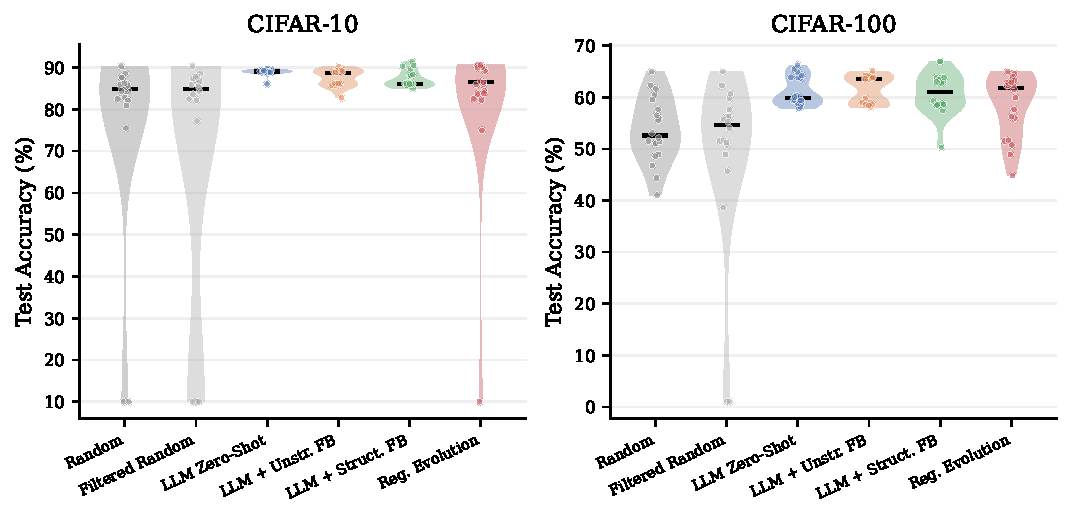
\includegraphics[width=\columnwidth]{fig1_violin.pdf}
  \caption{Violin plots with individual data points for all six conditions on
  CIFAR-10 (top) and CIFAR-100 (bottom).  LLM conditions form tight
  distributions; random baselines and REA show wide, often bimodal spreads.}
  \label{fig:violin}
\end{figure}

All three LLM conditions substantially outperform random search on both
datasets, with dramatically lower variance.  On CIFAR-10, LLM zero-shot achieves
$89.0\pm0.7$, compared to $77.3\pm22.6$ for random search, representing a
32-fold reduction in standard deviation.  On CIFAR-100, the LLM conditions
achieve means of 60.9--61.6, compared to $53.7\pm6.1$ for random search.

The filtered random baseline (A2) performs \emph{worse} than unfiltered random
($66.6$ vs.\ $77.3$ mean on CIFAR-10).  This counterintuitive result arises
because the heuristic filter inadvertently eliminates certain architecture
families, including some with few pooling layers that happen to perform
well~\citep{tan2019efficientnet}.  The filter shifts the parameter distribution
toward larger models ($778{\pm}612$K vs.\ $508{\pm}460$K;
Table~\ref{tab:arch}) without improving generalisation.  This result confirms
that the LLM's advantage cannot be attributed solely to generating well-formed
or appropriately sized designs, since a simple validity filter actually
\emph{degrades} random search performance.

Regularised evolution (E) exhibits high variance ($\text{std}{=}17.2$ on
CIFAR-10) due to bimodal behaviour under the 20-evaluation budget: some runs
inherit good designs from early mutations while others remain dominated by the
random initial population.  The best-case REA accuracy of 90.6\% is competitive
with all LLM conditions.

Crucially, feedback does not improve upon zero-shot generation.  On CIFAR-10,
both feedback conditions achieve lower mean accuracy than zero-shot ($87.6$ and
$87.2$ vs.\ $89.0$), and the structured case is statistically significant
(Section~\ref{sec:statcomp}).  On CIFAR-100, the three LLM conditions are
statistically indistinguishable (B vs.\ C: $p{=}0.61$, $d{=}{-}0.16$; B vs.\
D: $p{=}0.81$, $d{=}0.08$), indicating that feedback neither helps nor hurts
on the harder task.

\subsection{Statistical Comparisons}
\label{sec:statcomp}

Table~\ref{tab:stats_key} reports the seven pre-specified comparisons with
Bonferroni-corrected threshold $\alpha_{\mathrm{corr}}{=}0.0071$.

% -- Table 3: Statistical comparisons --
\begin{table}[t]
\centering\footnotesize
\caption{Pre-specified pairwise comparisons ($k{=}7$,
$\alpha_{\mathrm{corr}}{=}0.0071$).  Welch's $t$, Mann--Whitney $U$,
Cohen's $d$ [95\% CI].  $^*$\,significant after Bonferroni.  Positive $d$:
first condition higher.}
\label{tab:stats_key}
\begin{tabular}{@{}l ccc@{}}
\toprule
\multicolumn{4}{c}{\textit{CIFAR-10}} \\
\midrule
Comparison & $p_t$ & $p_U$ & $d$ \\
\midrule
A\,vs\,B   & .037  & ${<}.001^*$ & $-$0.71 \\
A2\,vs\,B  & .008  & ${<}.001^*$ & $-$0.94 \\
B\,vs\,C   & .007  & .042        & +0.93 \\
B\,vs\,D   & ${<}.001^*$ & $.002^*$ & +1.25 \\
A\,vs\,E   & .40   & .066        & $-$0.27 \\
\midrule
\multicolumn{4}{c}{\textit{CIFAR-100}} \\
\midrule
A\,vs\,B   & ${<}.001^*$ & ${<}.001^*$ & $-$1.53 \\
B\,vs\,C   & .606  & .787        & $-$0.16 \\
\bottomrule
\end{tabular}
\end{table}

On CIFAR-10, the comparison between zero-shot (B) and structured feedback
(D) yields a large effect size ($d{=}1.25$) that survives Bonferroni correction
on both the $t$-test ($p{<}0.001$) and $U$-test ($p{=}0.002$).  This is the
strongest evidence that feedback hurts.  The zero-shot vs.\ unstructured
feedback comparison (B vs.\ C) shows a similar direction ($d{=}0.93$), but the
$p$-values ($p_t{=}0.007$, $p_U{=}0.042$) place it at the margin: $p_t$
approximately equals $\alpha_{\mathrm{corr}}$, and $p_U$ does not survive
correction.  We therefore characterise B vs.\ C as \emph{marginal} and B vs.\ D
as \emph{significant}.  For random vs.\ zero-shot, the rank-based $U$-test
($p{<}0.001$) survives correction even when the $t$-test ($p{=}0.037$) does
not, reflecting the heavy-tailed random-search distribution where rank-based
tests have greater power.  Random search versus REA shows no significant
difference ($p_t{=}0.40$, $d{=}{-}0.27$).

On CIFAR-100, all LLM conditions significantly outperform random search with
large effect sizes ($d{=}{-}1.53$ for A vs.\ B, $p{<}0.001$).  Pairwise
comparisons among LLM conditions yield no significant differences (B vs.\ C:
$d{=}{-}0.16$, $p{=}0.61$), with confidence intervals crossing zero.  The
``feedback hurts'' finding is therefore specific to CIFAR-10, where the LLM
prior is already well-calibrated; on CIFAR-100 all LLM conditions perform
comparably.

\subsection{Convergence and Diversity}
\label{sec:diversity}

\begin{figure}[t]
  \centering
  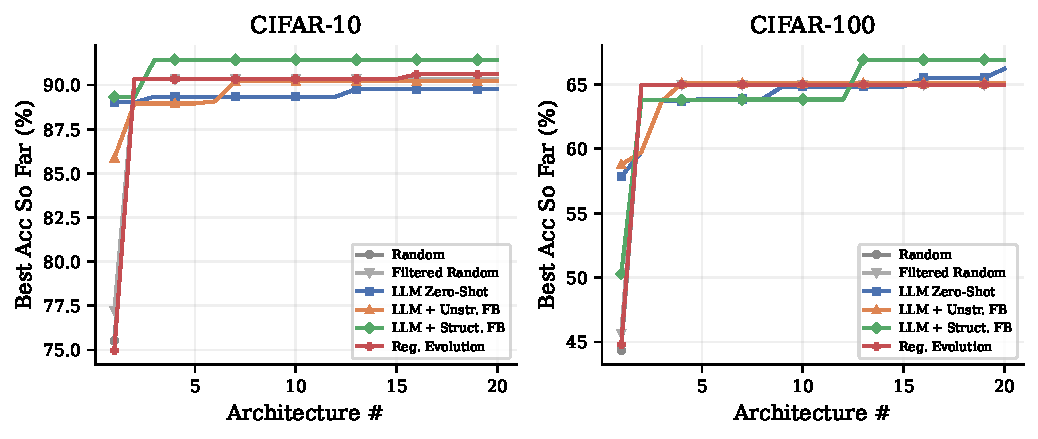
\includegraphics[width=\columnwidth]{fig2_convergence.pdf}
  \caption{Best-so-far test accuracy across 20 evaluations.  LLM conditions
  converge within 3--5 evaluations.  Random and REA show staircase patterns.}
  \label{fig:convergence}
\end{figure}

Figure~\ref{fig:convergence} shows best-so-far accuracy as a function of
evaluation number.  LLM zero-shot reaches near-optimal performance within
3--5 evaluations and shows minimal improvement thereafter, consistent with its
low diversity.  Random search and REA exhibit staircase improvement patterns.
The feedback conditions converge at an intermediate speed but never surpass the
zero-shot mean on CIFAR-10.

% -- Table 4: Architecture characteristics --
\begin{table}[t]
\centering\footnotesize
\caption{Architecture characteristics (CIFAR-10, seed\,42).  Par.\ = mean
parameters (K).  Blk = mean blocks.  Gap = generalisation gap (\%).
Eff.\ = accuracy per M parameters.  Div.\ = Jaccard distance.}
\label{tab:arch}
\begin{tabular}{@{}l rrcrrr@{}}
\toprule
Cond. & Par. & Blk & Gap & Eff. & Div. & Time\,(s) \\
\midrule
A       & 508 & 4.2 & 4.2 & 355 & .856 & 409 \\
A2      & 778 & 4.3 & 3.9 & 213 & .853 & 397 \\
B       & 511 & 4.0 & 6.0 & 174 & .022 & 219 \\
C       & 574 & 4.0 & 6.4 & 162 & .187 & 223 \\
D       & 727 & 4.0 & 6.8 & 137 & .268 & 236 \\
E       & 625 & 4.7 & 6.5 & 215 & .730 & 351 \\
\bottomrule
\end{tabular}
\end{table}

Table~\ref{tab:arch} reveals the most striking finding.  The zero-shot
condition exhibits a Jaccard distance of only $0.022$, indicating near-identical
architectures.  The parameter standard deviation is $0$K: every architecture
uses the same number of blocks ($K{=}4$), the same convolution types, the
same activation, the same normalisation, and the same skip-connection
configuration.  This is 39 times lower diversity than random search ($0.856$).
Yet this near-deterministic condition achieves the highest mean accuracy on
CIFAR-10.

\begin{figure}[t]
  \centering
  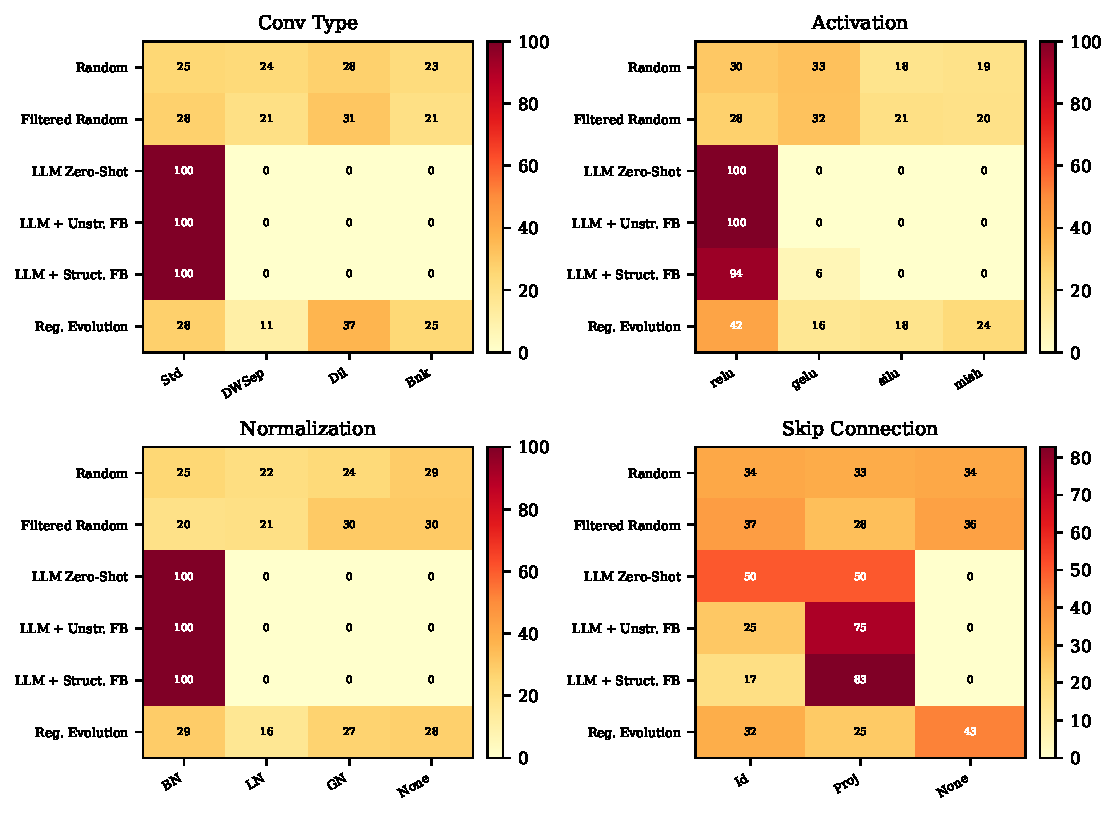
\includegraphics[width=\columnwidth]{fig4_design_heatmap.pdf}
  \caption{Design choice frequencies by condition.  Zero-shot (B) concentrates
  entirely on standard $3{\times}3$ convolutions, ReLU, and BatchNorm.
  Feedback conditions show slight broadening; random and REA distribute
  uniformly.}
  \label{fig:heatmap}
\end{figure}

Figure~\ref{fig:heatmap} details the specific design choices.  The zero-shot
condition (B) exclusively selects standard $3{\times}3$ convolutions (100\%),
ReLU activations (100\%), and BatchNorm normalisation (100\%), with skip
connections split evenly between projection (50\%) and identity (50\%).  This
template closely resembles the classical ResNet
block~\citep{he2016resnet,nair2010relu,ioffe2015batchnorm} rather than more
modern depthwise-separable or GELU-based
designs~\citep{howard2017mobilenets,ramachandran2017searching}.  The LLM's
prior is not only narrow but \emph{conservative}.

Unstructured feedback (C) maintains 100\% standard $3{\times}3$ and 100\% ReLU
but shifts skip connections toward projection (75\% vs.\ 25\% identity).
Structured feedback (D) introduces marginal variation: 99\% standard
$3{\times}3$ with 1\% other types, 94\% ReLU with 6\% GELU, and 100\%
BatchNorm.  By contrast, random search distributes roughly uniformly across
convolution types (28\% dilated, 25\% standard, 24\% depthwise-separable, 23\%
bottleneck) and activations (33\% GELU, 30\% ReLU, 19\% Mish, 18\% SiLU).
REA produces a mixed distribution (37\% dilated, 28\% standard, 11\%
depthwise-separable, 25\% bottleneck; 42\% ReLU, 24\% Mish, 16\% GELU, 18\%
SiLU).

\begin{figure}[t]
  \centering
  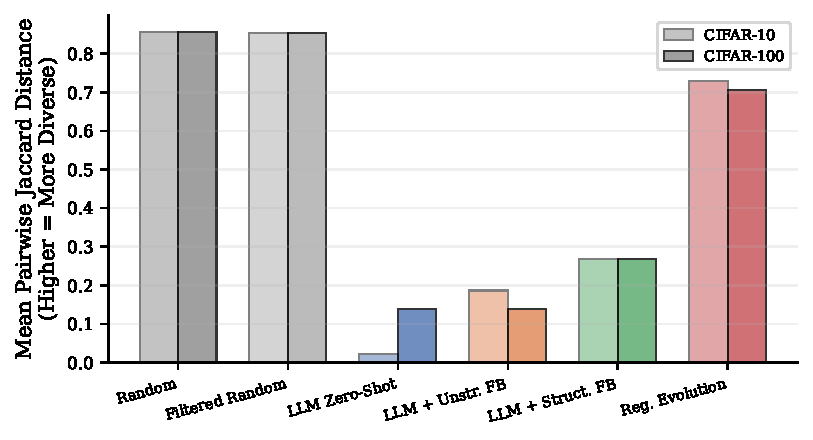
\includegraphics[width=\columnwidth]{fig6_diversity.pdf}
  \caption{Mean pairwise Jaccard distance by condition.  Feedback
  progressively increases diversity without improving accuracy.}
  \label{fig:diversity}
\end{figure}

Feedback increases diversity monotonically (Figure~\ref{fig:diversity}):
unstructured feedback raises the Jaccard distance to $0.187$ (8.5-fold over
zero-shot), and structured feedback further increases it to $0.268$.  This
diversification occurs because feedback prompts the LLM to deviate from its
default template.  However, these deviations move designs away from the strong
prior and into less well-characterised regions, resulting in lower mean accuracy
on CIFAR-10.  We term this the \emph{diversity--accuracy inversion}: the
opposite of what is typically assumed in search-based NAS, where greater
diversity aids exploration.

\begin{figure}[t]
  \centering
  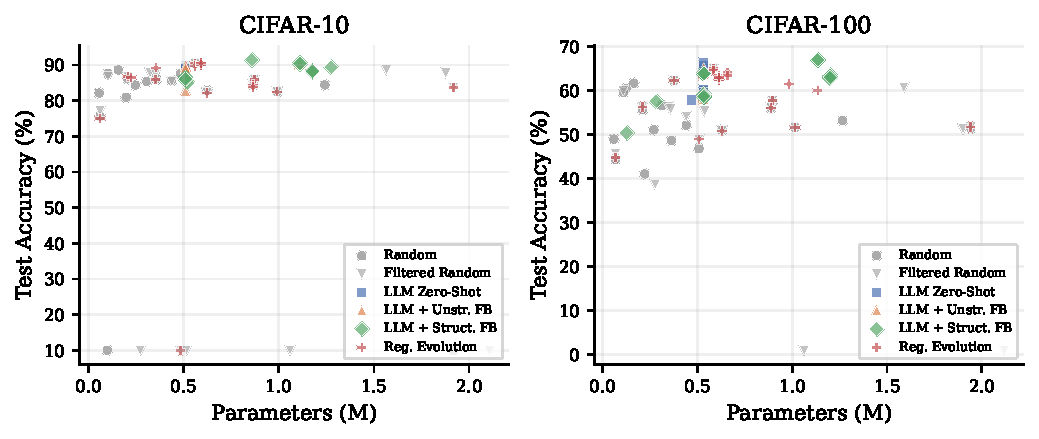
\includegraphics[width=\columnwidth]{fig3_param_accuracy.pdf}
  \caption{Parameters vs.\ test accuracy.  LLM conditions cluster
  tightly at 400--700K; random conditions span a much wider range.}
  \label{fig:scatter}
\end{figure}

Figure~\ref{fig:scatter} illustrates the parameter--accuracy relationship.
Feedback conditions produce progressively larger architectures (B: 511K, C:
574K, D: 727K), yet accuracy decreases.  The efficiency metric (accuracy per
million parameters) in Table~\ref{tab:arch} confirms this: condition~D achieves
the lowest efficiency (137) despite having the most parameters.

\subsection{Rank Stability and Training Dynamics}
\label{sec:rankstability}

% -- Table 5: Rank stability --
\begin{table}[t]
\centering\footnotesize
\caption{Rank stability: Spearman $\rho$ between validation accuracy at
epoch\,20 and final test accuracy (epoch\,50).}
\label{tab:rank}
\begin{tabular}{@{}l cc@{}}
\toprule
Condition & Spearman $\rho$ & $p$ \\
\midrule
A: Random        & 0.865 & ${<}0.001$ \\
A2: Filt.\ Rand. & 0.890 & ${<}0.001$ \\
B: Zero-Shot     & 0.462 & $0.040$ \\
C: Unstr.\ FB    & 0.708 & ${<}0.001$ \\
D: Struct.\ FB   & 0.651 & $0.002$ \\
E: Reg.\ Evol.   & 0.878 & ${<}0.001$ \\
\bottomrule
\end{tabular}
\end{table}

Table~\ref{tab:rank} reports Spearman rank correlations between validation
accuracy at epoch~20 and final test accuracy.  Random search and REA exhibit
high rank stability ($\rho{>}0.86$), indicating that early-stopping proxies
reliably identify the best architectures.  The zero-shot condition shows lower
stability ($\rho{=}0.462$, $p{=}0.040$), but this does not indicate poor
architecture quality; rather, it reflects the narrow accuracy range of
zero-shot designs (all between 87.8\% and 89.8\%), where small training
fluctuations reorder rankings.  The moderate $\rho$ for B suggests caution
regarding proposals to use early-epoch accuracy as a cheaper feedback signal
for LLM-designed architectures, since the signal-to-noise ratio is low when
the population is homogeneous.

\begin{figure}[t]
  \centering
  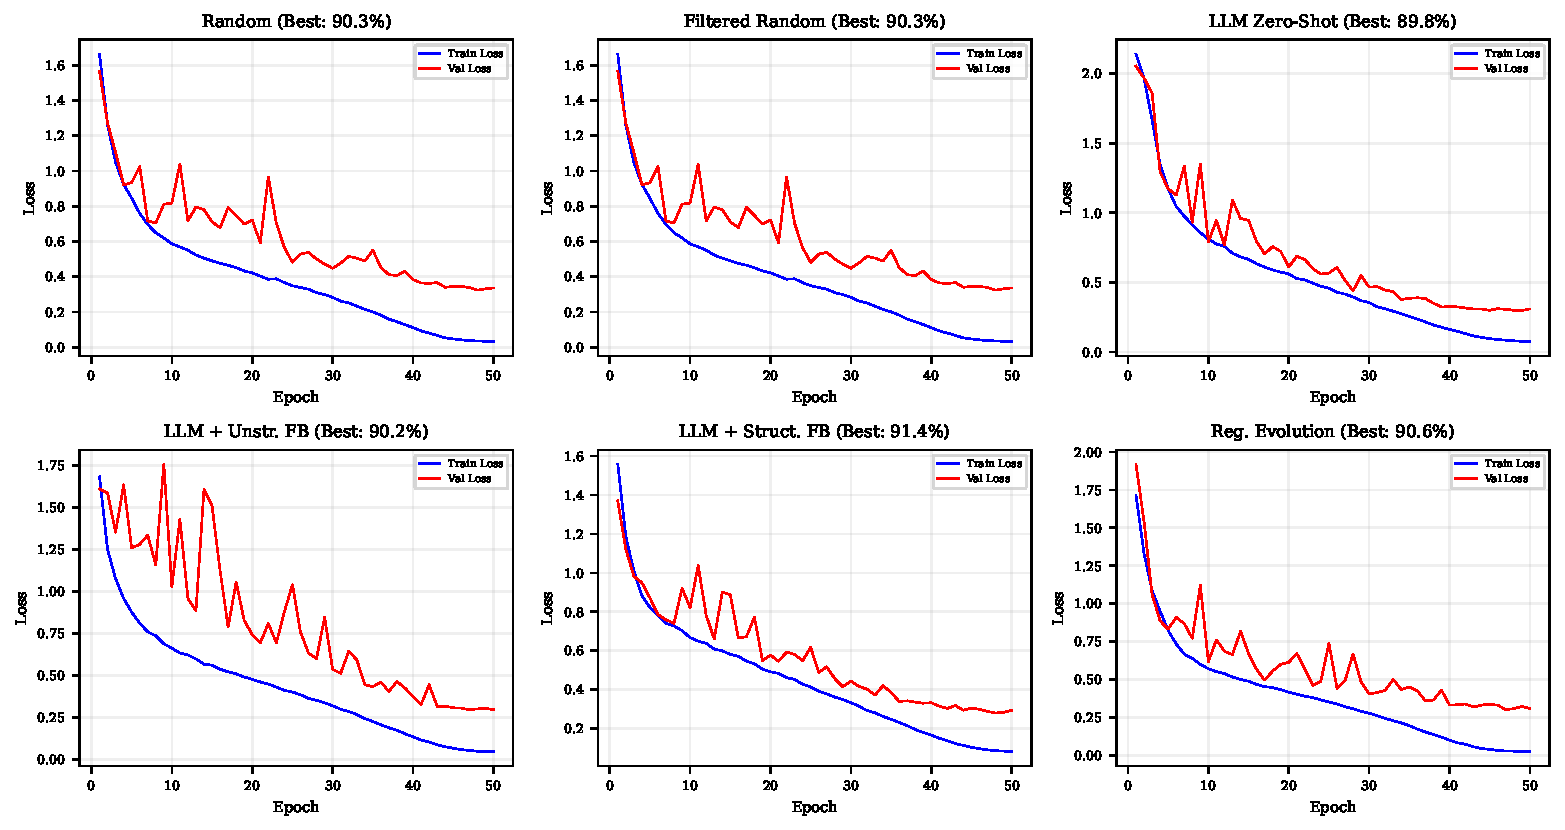
\includegraphics[width=\columnwidth]{fig5_training.pdf}
  \caption{Training curves for the best architecture per condition
  (CIFAR-10).  LLM architectures converge faster but exhibit a larger
  generalisation gap (Table~\ref{tab:arch}).}
  \label{fig:training}
\end{figure}

Figure~\ref{fig:training} shows training dynamics for the best architecture
from each condition.  All conditions achieve similar final training loss,
with LLM architectures converging slightly faster.  However, the generalisation
gap (Table~\ref{tab:arch}) is larger for LLM conditions ($6.0$--$6.8\%$) than
for random search ($4.2\%$), suggesting the LLM's template may benefit from
stronger regularisation.

\subsection{Transcript Analysis}

A key hypothesis was that the LLM would produce explicit causal reasoning about
architecture--performance relationships.  Analysis of all transcripts reveals
\emph{zero} causal attributions: Qwen3-1.7B outputs JSON specifications directly
with no accompanying reasoning text.  This null result is consistent with the
model's small size and limited chain-of-thought
capacity~\citep{wei2022chain,valmeekam2023planbench}.  Without causal
attribution, the model cannot translate performance metrics into targeted
modifications, which may explain the feedback interference effect.

\subsection{Replication}
\label{sec:replication}

Partial replication with seed~137 ($n{=}20$) on CIFAR-10 confirms the main
findings.  LLM zero-shot achieves $88.2\pm1.5$ (vs.\ $89.0\pm0.7$ at seed~42),
unstructured feedback achieves $88.3\pm1.3$ (vs.\ $87.6\pm1.9$), and random
search achieves $69.3\pm30.1$ (vs.\ $77.3\pm22.6$).  On CIFAR-100, the
seed-137 replication of zero-shot yields $61.1\pm2.5$ (vs.\ $61.1\pm2.7$ at
seed~42).  Pooling seeds 42 and 137 ($n{=}40$) gives zero-shot
$88.6\pm1.2$ and unstructured feedback $87.9\pm1.7$ on CIFAR-10, confirming a
stable advantage.  The LLM's superiority over random search and the absence of
feedback benefit replicate across seeds.

% ======================================================================
\section{Discussion}
\label{sec:discussion}
% ======================================================================

\subsection{The LLM as a Narrowband Prior}

Our results reframe the role of the LLM in architecture search.  Rather than
functioning as a flexible search agent that explores the design space and learns
from feedback, the LLM behaves as a \emph{strong but narrow prior}: it
concentrates probability mass on a single well-performing template and resists
meaningful exploration.  The zero structural variance of condition~B (parameter
std\,$= 0$K, Jaccard distance $0.022$) is remarkable.  Twenty independent
queries produce identical design choices: standard $3{\times}3$ convolutions,
ReLU, BatchNorm, and mixed projection/identity skips.  This template closely
resembles a canonical ResNet block~\citep{he2016resnet}, suggesting the LLM's
prior is shaped by the dominant architecture family in its training data.

The prior is well-calibrated in the sense that the default template achieves
high accuracy on both CIFAR-10 and CIFAR-100, but it is brittle: perturbations
induced by feedback degrade rather than improve performance on the easier task.
The practical implication is clear: rather than investing compute in sequential
refinement, practitioners should sample a small number (3--5) of independent
zero-shot architectures and select the best by validation accuracy.

\subsection{Why Does Feedback Hurt?}

We identify three mechanisms for the feedback interference effect.  First, the
LLM may lack the causal reasoning capacity to translate performance metrics into
actionable modifications.  The null transcript analysis supports this: without
explicit reasoning, the model processes feedback as a generic signal to ``change
something'' rather than targeted guidance.

Second, feedback may trigger a \emph{novelty bias} in which the instruction to
``improve'' is interpreted as ``change.''  The diversity data support this:
Jaccard distance increases monotonically from zero-shot ($0.022$) through
unstructured ($0.187$) to structured feedback ($0.268$).  More information in the
feedback paradoxically leads to more deviation from the prior.

Third, with multiple components changing between iterations and only 20
evaluations, the LLM cannot isolate which changes caused performance
differences.  Structured edit prompts constraining the model to change at most
one component per iteration~\citep{madaan2023selfrefine} could mitigate this
confound and represent a promising direction for future work.

\subsection{Training Budget Confound}

An important caveat concerns the fixed training budget.  Feedback conditions
produce larger architectures (B: 511K, C: 574K, D: 727K), which may require
more epochs to converge.  If anything, this bias favours feedback conditions:
larger models have greater capacity and should benefit from 50 epochs of
training.  Yet accuracy still decreases.  The generalisation gap data
(Table~\ref{tab:arch}) show that larger LLM architectures overfit more
($6.8\%$ gap for~D vs.\ $6.0\%$ for~B), indicating the accuracy loss is not
explained by underfitting alone.  Nevertheless, the confound is real: future
work should explore adaptive training schedules that account for model size.

\subsection{Limitations}
\label{sec:limitations}

Several limitations qualify our findings.  \textbf{(i)~Single small LLM.}  We
use Qwen3-1.7B-4bit; larger models with stronger reasoning
capabilities~\citep{openai2023gpt4} may respond differently to feedback and
produce richer priors.  The narrowband prior finding may be model-size
dependent, with larger models exhibiting broader priors that benefit more from
refinement.  \textbf{(ii)~Search space scope.}  Our custom CNN space on
CIFAR-10/100 provides maximal experimental control but limits generalisability.
Evaluation on NAS-Bench-201~\citep{dong2020nasbench201} would enable zero-noise
comparisons and is a natural next step.  \textbf{(iii)~REA budget.}  Twenty
evaluations is modest for evolutionary search; the high REA variance reflects
this limitation.  \textbf{(iv)~Transcript null result.}  The small model's
minimal text output prevents us from characterising its reasoning process.
\textbf{(v)~Prompt design.}  We do not explore structured edit prompts
(\eg ``change at most one component'') that might preserve the LLM's prior
while enabling targeted exploration.  \textbf{(vi)~Fixed 50-epoch budget.}
Larger feedback-condition architectures may benefit from longer training.
\textbf{(vii)~Partial replication.}  Seed~137 covers four of six conditions;
full multi-seed replication would strengthen the conclusions.

% ======================================================================
\section{Conclusion}
\label{sec:conclusion}
% ======================================================================

We have presented a controlled study of LLM-guided neural architecture design
that isolates the effect of performance feedback on generation quality.  A
small, quantised LLM (Qwen3-1.7B-4bit) encodes a strong prior over a single
conservative template (standard $3{\times}3$ convolutions, ReLU, BatchNorm),
producing 20 structurally identical designs that significantly outperform random
search ($89.0$ vs.\ $77.3$ on CIFAR-10, $61.1$ vs.\ $53.7$ on CIFAR-100)
while reducing variance by more than 30-fold.  Structured feedback significantly
disrupts this prior on CIFAR-10 ($d{=}1.25$, $p{<}0.001$ after Bonferroni
correction), increasing diversity without improving accuracy.  On CIFAR-100,
feedback and zero-shot perform comparably ($d{=}{-}0.16$, $p{=}0.61$).  These
findings challenge the assumption that self-refinement universally improves
LLM-based design and suggest that, under fixed compute budgets, parallel
zero-shot sampling is the preferred strategy.  Future work should investigate
whether larger models can productively leverage feedback, whether structured
edit constraints preserve the prior while enabling exploration, and whether
these findings generalise to cell-based and transformer search spaces.

% ======================================================================
\subsection*{Impact Statement}
% ======================================================================

This work studies the automation of neural architecture design using language
models.  Our finding that zero-shot generation often suffices suggests a path
toward more compute-efficient design workflows, reducing the environmental cost
of NAS.  We see no direct negative societal impacts from this methodology
research, but acknowledge that improved NAS techniques could accelerate
development of AI systems requiring careful ethical consideration.

% ======================================================================
\subsection*{Reproducibility}
% ======================================================================

All code, prompts, configuration files, random seeds, and analysis scripts will
be released in a public repository upon acceptance.  The complete JSON schema,
prompt templates, and per-architecture results are provided in the appendices.

% ======================================================================
%  REFERENCES
% ======================================================================
\bibliography{references}

% ======================================================================
%  APPENDIX  (uncounted pages)
% ======================================================================
\newpage
\appendix

\section{Prompt Templates}
\label{app:prompts}

\subsection{System Prompt (All LLM Conditions)}

\begin{quote}\small\ttfamily
You are an expert neural network architect. Your task is to design CNN
architectures for image classification. You must output a valid JSON object
conforming to the schema below. Design architectures that balance accuracy,
parameter efficiency, and trainability.
\end{quote}

The system prompt is followed by the full JSON schema (Appendix~\ref{app:schema})
and a task description specifying the target dataset and input dimensions.

\subsection{Unstructured Feedback (Condition C)}

After each evaluation:

\begin{quote}\small\ttfamily
Your previous architecture achieved \{val\_acc\}\% validation accuracy
with \{params\}K parameters. Please design an improved architecture.
\end{quote}

\subsection{Structured Feedback (Condition D)}

A JSON report is appended containing: \texttt{val\_accuracy},
\texttt{train\_loss\_final}, \texttt{convergence\_rate},
\texttt{param\_count}, and the full \texttt{architecture} specification of the
previous design.

\section{JSON Schema}
\label{app:schema}

The architecture schema includes: \texttt{num\_blocks} (2--6),
\texttt{blocks} (array, each with \texttt{conv\_type}, \texttt{channels},
\texttt{kernel\_size}, \texttt{activation}, \texttt{norm}, \texttt{pooling}),
\texttt{skip\_type} (identity/projection/none), \texttt{classifier}
(\texttt{num\_layers}, \texttt{dropout}), and \texttt{global\_pooling}
(avg/max).  Convolution types: standard, depthwise-separable, dilated,
bottleneck.  Activations: ReLU, GELU, SiLU, Mish.  Normalisation: batch,
layer, group, none.

\section{Full Statistical Tables}
\label{app:fullstats}

The seven pre-specified comparisons and their full statistics are reported in
Table~\ref{tab:stats_key}.  Additional exploratory comparisons include:
A\,vs\,C on CIFAR-100 ($p_t{<}0.001$, $p_U{<}0.001$, $d{=}{-}1.63$,
significant), B\,vs\,D on CIFAR-100 ($p_t{=}0.81$, $p_U{=}0.39$, $d{=}0.08$,
not significant), and A\,vs\,E on CIFAR-10 ($p_t{=}0.40$, $p_U{=}0.066$,
$d{=}{-}0.27$, not significant).

\section{Per-Seed Breakdown}
\label{app:perseed}

\begin{table}[h]
\centering\footnotesize
\caption{Per-seed results for replicated conditions.}
\label{tab:perseed}
\begin{tabular}{@{}l l l r@{$\,\pm\,$}l@{}}
\toprule
Condition & Dataset & Seed & \multicolumn{2}{c}{Mean$\pm$Std} \\
\midrule
A: Random          & C-10  & 42  & 77.3 & 22.6 \\
A: Random          & C-10  & 137 & 69.3 & 30.1 \\
B: Zero-Shot       & C-10  & 42  & 89.0 & 0.7 \\
B: Zero-Shot       & C-10  & 137 & 88.2 & 1.5 \\
C: Unstr.\ FB      & C-10  & 42  & 87.6 & 1.9 \\
C: Unstr.\ FB      & C-10  & 137 & 88.3 & 1.3 \\
B: Zero-Shot       & C-100 & 42  & 61.1 & 2.7 \\
B: Zero-Shot       & C-100 & 137 & 61.1 & 2.5 \\
\midrule
\multicolumn{5}{c}{\textit{Pooled ($n{=}40$, seeds 42+137)}} \\
\midrule
B: Zero-Shot       & C-10  & all & 88.6 & 1.2 \\
C: Unstr.\ FB      & C-10  & all & 87.9 & 1.7 \\
B: Zero-Shot       & C-100 & all & 61.1 & 2.6 \\
A: Random          & C-10  & all & 73.3 & 26.9 \\
\bottomrule
\end{tabular}
\end{table}

Seed-137 results confirm all qualitative findings.  Random conditions show
high variance ($\text{std}{>}27$) across seeds, and the LLM advantage
persists.  Pooled zero-shot CIFAR-10 ($88.6\pm1.2$, $n{=}40$) confirms the
stability of the main finding.

\section{Channel Width Distributions}
\label{app:channels}

\begin{figure}[h]
  \centering
  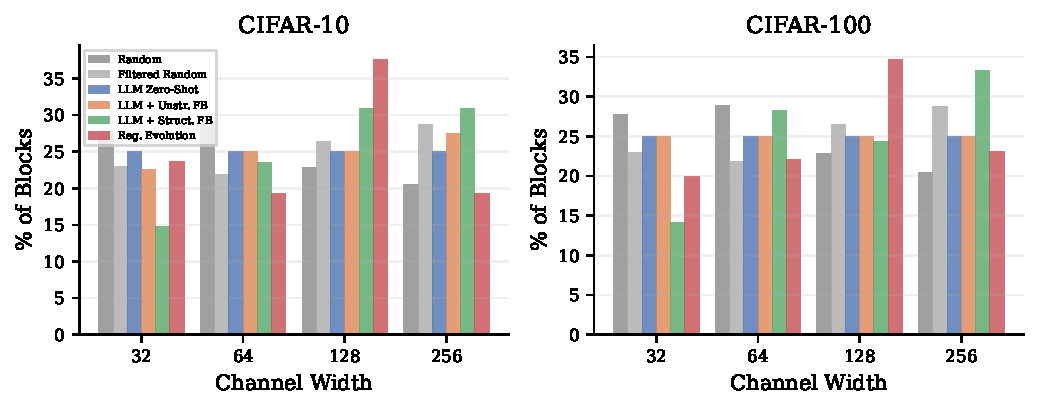
\includegraphics[width=\columnwidth]{fig7_channels.pdf}
  \caption{Channel width distributions across conditions.  LLM conditions
  concentrate on 32--128 channels; random conditions span the full 16--256
  range.}
  \label{fig:channels}
\end{figure}

\end{document}
